\subsection{Modeling}

	The development process of the PDSurvey platform was inspired and influenced by the concept of extreme programing\footnote{\url{http://www.extremeprogramming.org/rules.html} (last visited on April 10, 2015)}, making iterative improvements, and working agile and user centered. First user stories were written and assessed in a small group\footnote{\url{http://www.tigertech.de/wie-schreibe-ich-eine-gute-user-story-und-was-ist-das-uberhaupt/} (last accessed April 10, 2015). The next step was to transfer these stories to user models, describing in detail which functionality the stakeholders of PDSurvey are supposed to have. Later a first software architecture and software model was built. Dependencies between models were defined and the model was continuously refined and improved throughout the development phase. The last phase included screen designs, getting a clear view of what the interface might later look like.

	% Mongoose + REST API
	The model for the \textit{PDSurvey} platform is maintained with Mongoose. Angular.js builds its model from the REST API, and maps all changes via dynamic two-way-binding to it's scope. The REST API is provided by the Node.js server, which maps all incoming requests through an Express router to the corresponding Mongoose models. Thus all changes to the model originate from Mongoose.

	% User roles
	Currently three user roles are implemented for the platform: an \textit{admin} role (for administrators), an \textit{expert} mode (with a mapping of n surveys to m displays), and a \textit{novice} mode (with a simplified interface).

	% REST API
	The development of the REST API was influenced by current best practices \cite{Sahni2015RESTAPI, TutsPlus2015RESTAPI, hughes2012einfuhrung}. The API is separated into logical resources, while each resource gets manipulated through an HTTP request. For public access GET and POST is defined, for authenticated users also PUT and DELETE. For a more information about PDSurvey's REST API refer to the documentation (see Appendix \ref{appendix:documentation}).

	% Our Software Model
	The software model is modeled in Mongoose and stored as MongoDB collections. There are the following collections: \textit{Question, QuestionType, Response, Category, Surveys, User, DisplayModel, Display, Campaign, Context, User}. 
	Of special interest are the following four collections: Surveys, Display, Campaign and Responses (see figure \ref{fig:4-dependency-campaign}).

\begin{figure}%[btph]
    \begin{center}
        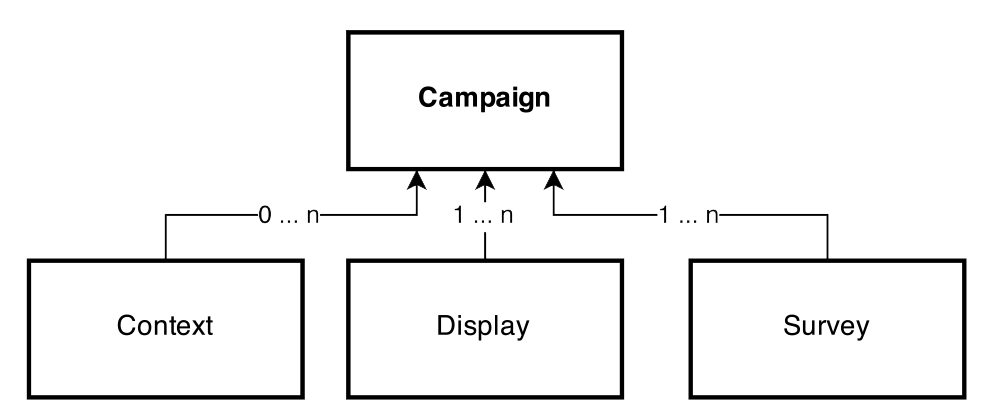
\includegraphics[width=.8\columnwidth]{img/4_implementation/4-dependency-campaign}
    \end{center}
 % \begin{center}\LARGE [BILD]\end{center}
 \caption{Campaign model dependencies}
 \label{fig:4-dependency-campaign}
\end{figure}


	\paragraph{Surveys:} Questionnaires are the foundation of PDSurvey, consisting of multiple sections, which in turn are made up of multiple questions. Each question is of a corresponding question type and every questionnaire belongs to a category. This allows questionnaires to be filtered based on certain research questions. Additionally we added the ability to set surveys \textit{private} (by default), \textit{shared} (for sharing with other users), \textit{standardized} (scientifically recognized), or \textit{pending} (waiting for review, to be shared). Every survey is assigned to an individual user of the platform, with the aim of reuse and standardization of questionnaires.

	\textbf{TODO ueberlegen ob ich den letzten Absatz Surveys oder Questionnaires nennen mag}


	\paragraph{Display:} In the display collection all displays connected to the PDSurvey platform are contained. To allow for an evaluation across multiple display models and based on the context of the displays, the display model and a static and/or dynamic context is assigned to it.

	\paragraph{Campaign:} Campaigns resemble the most integral part of the platform, since they glue all of the pieces together and allow the distribution of surveys to public display networks. A campaign consists of displays and surveys, and creates the mapping of the questionnaires to public displays. Additionally to each of those mapping an individual context can be assigned, enabling the later comparison of results in between the public displays.

	\paragraph{Response:} All responses made to each survey are logged in the Response collection. The queries are logged individually per user, per display and per campaign. This model will be the base for further extensions, such as the automatic evaluation of the survey responses and the comparison in between different displays inside one display network. This enables to find out which properties of a display might cause certain effects.

	\paragraph{Context:} One of the benefits of creating this survey platform is the ability to collect and evaluate large amounts of data, without increasing the workload on the human component for conducting and evaluating the responses. The idea is to collect a large number of responses from a variety of displays in various settings, and assigning a specific context to every display connected to PDSurvey. Once enough data is collected, the results can be evaluated and compared in between the displays. Interesting questions for analysis would be, which role the context plays on how the users respond to the display, when running identical software settings on the displays, but only varying the context (position, size of display, surrounding environment of the display, positioning it outdoors or indoors, influence of the weather, type of building it is positioned in).

